\documentclass{article}
\usepackage{graphicx}
\usepackage[utf8]{inputenc}

\title{A report regarding the optimization of 2D plus MOT using Machine learning}
\author{Xuhui Chen}
\date{August 2019}

\begin{document}

\section{Machine Learning Algorithm and its implementation}
Optimization algorithms commonly used are Gaussian process and Genetic Algorithm. Both of them are capable of optimizing the output of a unkown function when the evaluation cost, the running time of the function, is high.

Gaussian process ultilizes Bayesien Process and assumes each set of data we collect is normally distributed. It will suggest where the next data point to evaluate and will eventually lead to the global maximum in an ideal situation.

Genetic algorithm simulates what happens in real world. It considers each set of parameters as an "individual", and simulates the mating and mutation of the individual to select the best individual possibles. In this way, the "population", a group of individuals, will evolve and provide the best solutions to the optimization problem.

In this code, both method has been implemented. Gaussian process is implemented using GpyOpt library, and the Genetic Algorithm is with the help of "deap" library.

\subsection{Optimization Goal}

Here the optimization goal is to maximize the capture ratio of the 2D plus MOT, ignoring all other parameters, such as average velocity of the captured atoms. The parameters being optimized involve the height of the cooling beam with respect to the pushing beam, the detuning and e-radius of the cooling/pushing beams and the gradient of the magnetic field.

\subsection{Implementation of the machine learning combined two algorithms}

After some tries, I found out that the Gaussian process is not producing a lot of meaningful results. While some of the results are impressive and better than what I manually chose, many of the setups suggested by gaussian process produce zero capture ratio. A typical diagram of the evolution is given in the following graph.
\begin{figure}
	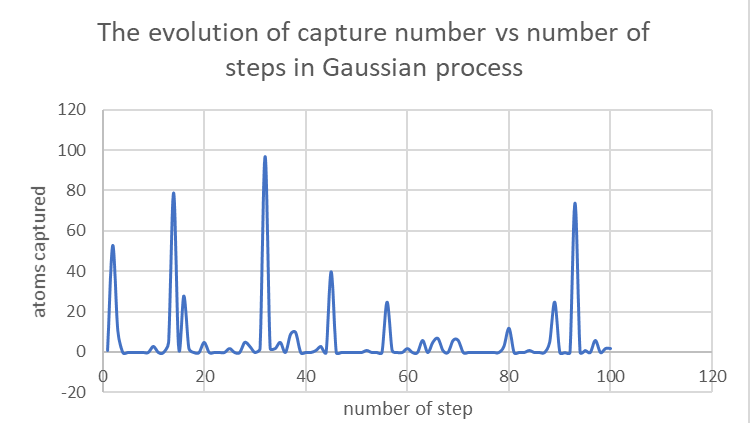
\includegraphics[width=\columnwidth]{GP.png}
	\caption{number of captured atoms as gaussian process progesses}
\end{figure}

The reason for this strange behaviour is that the nature of the simulation invalidate the assumption of gaussian process: the set of data collected will be gaussian. It is due to the fact that the paratmeters being optimized are strongly related to each other and have a lot of the local maximums (this will be explained in more details in the following chapters). Moreover, a lot of the parameters combinations produce zero capture ratio and meanings combinations often form in clusters, making gaussian process more challenging.

Thus, a different approach is taken. Instead of solely relying on the gaussian process, I combine the two machine learning algorithms and use gaussian process as a sample generator. As it is shown in the previous graph, gaussian process is capable to produce some meaningful results, and those results are recorded and then use as the population of the genetic algorithm. The rest of the optimization will be done in genetic algorithm.

Genetic algorithm is especially suitable for this optimization task due to the facts that many parameters are only meaningful when it is considered together with the other parameters, e.x. gradient of quodrupole field & detuning. It is very similar to how biological genes function, and  genetic algorithm is based on biological evolution. To be more specific, in genetic algorithm, when two individuals are mating, a process during which part of their genes are interchanged, they may exchanged a pair of strongly coupled parameters. As a result, the "mating" process may lead to the meaningful exchanges during which the a group of paramters that are strongly related, instead of one single parameter, get altered.

\Section{ Result }





\end{document}